\documentclass[a4paper,oneside,8pt]{extarticle}
\usepackage{style}  % importaj vse package ki jih rabis

\graphicspath{ {./img/} }
\addbibresource{bibliography.bib}


\newcommand{\Title}{Sistemska Programska Oprema - Latex Compiling}
\newcommand{\Author}{Rok Kos}
\title{\Title}
\author{\Author}
\date{\today}
\hypersetup{pdftitle={\Title}, pdfauthor={\Author}, pdfcreator={\Author}, pdfproducer={\Author}, pdfsubject={}, pdfkeywords={}}  % setup pdf metadata

\pagestyle{empty}              % vse strani prazne
\setlength{\parindent}{0pt}    % zamik vsakega odstavka
\setlength{\parskip}{10pt}     % prazen prostor po odstavku
% \setlength{\overfullrule}{30pt}  % oznaci predlogo vrstico z veliko črnine

\newcommand{\latex}{\LaTeX\xspace}
\newcommand{\tex}{\TeX\xspace}

\begin{document}
\title{\Title}

\author{\Author}

\maketitle

\pagebreak

\tableofcontents

\listoffigures

\pagebreak

\section{Introduction}
So in this seminar, I will present how compiling in \latex works. This is the world's most popular typesetting system for scientific and technical documentation.

From now on when I will use word \latex I will refer to \LaTeX2$\varepsilon$ and not old \LaTeX2.09 or new LaTeX3 which is currently in development.

But first, we need to clear some things first. \latex is built on top of \tex. \tex is low-level typesetting system/formatting engine created by Professor Donald Knuth. 
 \latex provides all the macros (written in \tex) for formatting that are easy to use.  

So basically you can imagine that \latex is more focused on content and \tex is more focused on formatting text and making it look the way you want.

\subsection{Distributions and Compilers}
\tex distribution is basically toolset that allows you to compile your \latex document. It consists of a set of programs and each major OS has it \cite{Latex_project_distributions} \cite{Overleaf_Compilers}.
Some popular and maintained distributions:
\begin{itemize}
	\item \textbf{TeX Live} for Linux and other UNIX-like systems 
	\item \textbf{MacTeX} redistribution of TeX Live for macOS 
	\item \textbf{MiKTeX} for Windows 
	\item \textbf{proTeXt} is based on MiKTeX 
\end{itemize}

and there are also some that are not actively maintained \cite{Old_Distributions}:
\begin{itemize}
    \item \textbf{teTeX} for Linux and other UNIX-like systems
    \item \textbf{fpTeX} for Linux and other UNIX-like systems 
    \item \textbf{emTeX} for MS-DOS and OS/2
    \item \textbf{gwTeX} or macOS 
    \item \textbf{OzTeXor} macOS
    \item \textbf{AmigaTeX} for the Amiga
    \item \textbf{PasTeX} for the Amiga
\end{itemize}

Each of these distributions supports compilers that can output three types of documents:
\begin{itemize}
	\item \textbf{DVI} - Device independent file format. This is usualy output of \textbf{latex} compiler 
	\item \textbf{PDF} - Portable Document Format. This is output of \textbf{pdflatex} compiler
	\item \textbf{PS} - PostScript format. We get this by compiling .tex file  first to DVI or PDF and then converting it to PS. 
\end{itemize}

Some other compilers that also exist are XeLaTeX and LuaLaTeX.

\subsection{Getting the desired output}

So how do we get our text from document.tex to PDF or DVI form? I will show an example on Linux with \tex Live distribution.
It's easy as typing a command into the terminal (under the condition that you previously setup you distribution correctly)
So we type in 
\begin{lstlisting}[language=bash]
    $ pdflatex document.tex
\end{lstlisting}

for PDF output or

\begin{lstlisting}[language=bash]
    $ latex document.tex
\end{lstlisting}

for DVI output.\\

You might ask why I am doing this seminar if it's so easy. That I will explain this in the following chapters.

But before we continue I will just add one picture to show with which commands you can get which output. See the figure \ref{fig:latex-compiling-flow} below.
\begin{figure}[h]
    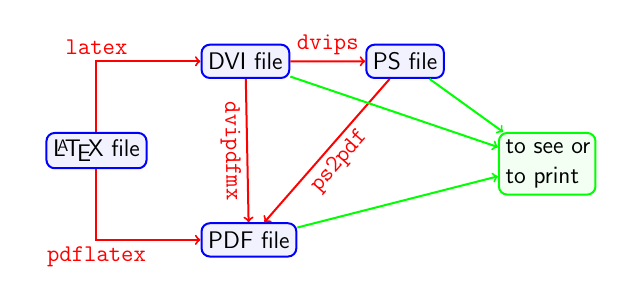
\includegraphics[width=\textwidth]{Latex-file-flow.png}
    \caption{Latex compiling flow (from site \cite{Overleaf_Compilers}) }
    \label{fig:latex-compiling-flow}
\end{figure}

\section{Compiling process}

In this section, I will talk more about what happens when you compile your \latex document. By this I mean when you use commands like pdflatex, biber etc. 

When you run pdflatex command compiler goes through the whole document and searches for tags/commands like \verb|\label|, \verb|\ref|, \verb|\cite|, \verb|\include|, \verb|\input|, \verb|\section|, subsection etc. (It also searches for other commands that define formatting, include different packages, create graphs and other things, but this is not so important for compiling). And when it gets to the end of the document (we call this page ship out) it produces several files \cite{Dickimaw_Books}:
\begin{itemize}
	\item \textbf{.log} file - this file will be created after each compilation. It holds information about which packages and file have been included (with information like version of package, date etc.). Log file will also record if there is any error or warning. Besides that, it will also contain some general messages and information about the compiled document. This is the file you should first look if anything goes wrong.
	\item \textbf{.aux} file - This is an auxiliary file which contains all the information for cross-referencing. In this file goes all the information about \verb|\label|, \verb|\ref| and other commands that I mentioned previously. You can look at this as \textbf{Symbol table} (SYMTAB) from SIC assembler. If you delete this file then you will need to run pdflatex command twice each time (but more about this later).
	\item \textbf{.toc} file - Table of content file
	\item \textbf{.lof} file - List of figure file
	\item \textbf{.lot} file - List of tables  file
\end{itemize}

Additionally, if you use bibtex or biblatex you could also get some file associated with bibliography like .bbl, .bcf, .blg. They have same purpose as .log, .aux and .toc files.

I will focus on useful and most common file that you will get are .log and .aux files. Other files I will just briefly go through. 

\subsection{Log Files in \latex}


Log files are a source of information about what happened during the compilations.  I will present some of the information that you can find in log file \cite{understanding_the_log_file}.

\begin{enumerate}
	\item \textbf{Compiler information} - This first line in .log file. It information about which compiler you are using, which version, which \tex distribution you are using and timestamp. \\
          One example from my laptop using pdflatex compiler:\\
            \begin{markdown-block}
                This is pdfTeX, Version 3.14159265-2.6-1.40.18 (TeX Live 2017) (preloaded format=pdflatex 2018.7.17)  14 JAN 2019 12:54
                entering extended mode
            \end{markdown-block}
          and one other example using xelatex compiler from \cite{understanding_the_log_file}:
            \begin{markdown-block}
                This is XeTeX, Version 3.1415926-2.3-0.9997.5 (Web2C 2011)  
            \end{markdown-block}

    \item \textbf{Included packages} - For every package that you include in your document compiler will output line that tells the name of the package, version of the package you are using, date of this version, where this package is on your system and a short description of the package. 
    Example:\\
        \begin{markdown-block}
            (/usr/share/texlive/texmf-dist/tex/latex/amsmath/amsmath.sty\\
            Package: amsmath 2016/06/28 v2.15d AMS math features
        \end{markdown-block}

    \item \textbf{Warnings} - This will usually occur with cross-referencing. Some of the cases would be:
        \begin{itemize}
            \item undefined \verb|\ref| - This means that you have \verb|\ref| that is pointing to non existing \verb|\label|. The solution for this is that you add missing \verb|\label|. \\
                You would warning like this:
                \begin{markdown-block}
                    LaTeX Warning: Reference \verb|`fig:test_123'| on page 4 undefined on input line 121.
                \end{markdown-block}

                The compiler, in this case, would output two questions marks in your PDF like this:
                \begin{figure}[h]
                    \centering
                    
\includegraphics[width=0.5\textwidth]{UndefinedRef.png}
                    \caption{Undefined Ref}
                    \label{fig:UndefinedRef}
                \end{figure}

                You can try this if you run compile Primer00.tex in the repository. Or you can use a handy script that I wrote and just type:
                \begin{lstlisting}[language=bash]
                    $ ./CompilePrimer.sh Primer00
                \end{lstlisting}
            
            \item \verb|\label| not found in .aux file - This happens when we first run our compiler the .aux file is empty and it doesn't have any data. When trying to reference a label it doesn't find any reference in .aux file. The solution for this is to again run pdflatex command and by doing this compiler will find a reference. It will output same warning as with undefined \verb|\ref| . I will show quick example here:\\
                  This is the first run of pdflatex:\\
                  \begin{figure}[h]
                    \centering
                    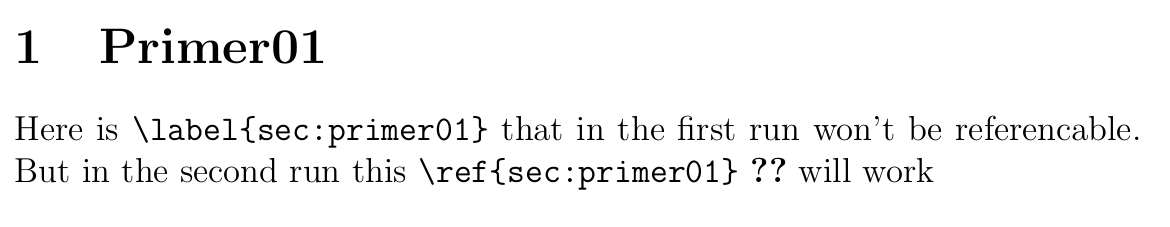
\includegraphics[width=0.5\textwidth]{FirstRun.png}
                    \caption{First Run}
                    \label{fig:FirstRun}
                \end{figure}
                
                  This is the second run:\\
                  \begin{figure}[h]
                    \centering
                    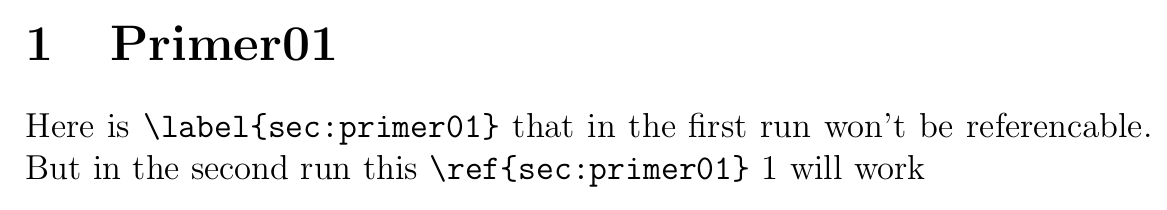
\includegraphics[width=0.5\textwidth]{SecondRun.png}
                    \caption{Second Run}
                    \label{fig:SecondRun}
                  \end{figure}

                  You can also try out with Primer01 that I attached with CompilePrimer.sh script.


            \item missing reference when citing bibliography - This is due too wrong naming in \verb|\cite| command or in missing reference .bib file or not running bibtex/biber command before pdflatex. The solution is to either correct name in \verb|\cite| command or to add an entry in .bib file or to run commands in this sequence pdflatex -> bibtex/biber -> pdflatex -> pdflatex.\\
            The warning message will look something like:\\
            \begin{markdown-block}
                LaTeX Warning: Citation \verb|'John_Doe'| on page 1 undefined on input line 13.\\
                \\
                .\\
                .\\
                .\\
                \\
                LaTeX Warning: There were undefined references.\\
                \\

                Package biblatex Warning: Please (re)run Biber on the file:\\
                (biblatex)                LatexCompiling\\
                (biblatex)                and rerun LaTeX afterwards.\\
            \end{markdown-block}
            The output of compiled PDF after first will be:\\
            \begin{figure}[H]
                \centering
                
\includegraphics[width=0.5\textwidth]{CitationWarning01.png}
                \caption{Citation Warning first run}
                \label{fig:CitationWarning01}
            \end{figure}
            Here you can see that citations that are missing will be in brackets and the name of citations will be in this brackets ( \verb|[citation_ref]| ).\\
            In the second run (after doing bibtex/biber -> pdflatex -> pdflatex) we got desired output.\\
            \begin{figure}[H]
                \centering
                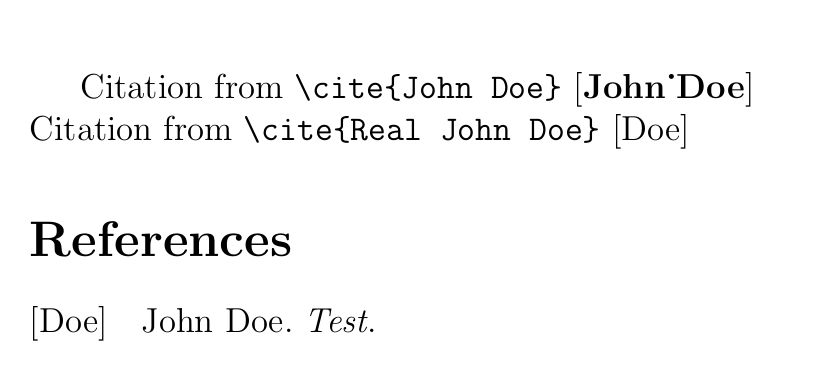
\includegraphics[width=0.5\textwidth]{CitationWarning02.png}
                \caption{Citation Warning second run}
                \label{fig:CitationWarning02}
            \end{figure}
            We had the reference in .bib file about Real John Doe. So you can see that compiler found the reference. As for John Doe, it stayed the same because we didn't put in the reference in .bib file. \\

            You can also try out with Primer02. 

        \end{itemize}


    \item \textbf{Statistics} - At the end of each file there will be statistics on document and pdf that can look something like this:
        \begin{markdown-block}
            Here is how much of TeX's memory you used:\\
            28649 strings out of 493064\\
            455396 string characters out of 6138159\\
            930333 words of memory out of 5000000\\
            31707 multiletter control sequences out of 15000+600000\\
            52065 words of font info for 88 fonts, out of 8000000 for 9000\\
            1137 hyphenation exceptions out of 8191\\
            \\
            Output written on LatexCompiling.pdf (5 pages, 112356 bytes).\\
            PDF statistics:\\
            107 PDF objects out of 1000 (max. 8388607)\\
            92 compressed objects within 1 object stream\\
            19 named destinations out of 1000 (max. 500000)\\
            46 words of extra memory for PDF output out of 10000 (max. 10000000)\\
        \end{markdown-block}

\end{enumerate}


\section{Auxiliary Files in \latex}

As we mentioned before in Auxiliary file (.aux) there is information for cross-referencing. This is probably the most interesting and crucial part of compiling. Latex compiler will open this file before it will start parsing main .tex file. By doing this it will extract all the info for cross-referencing. When parsing document it will try to resolve all the references and at the end of the file, it will write to .aux file all the new references and values of this references. It's similar to the process 2-phase SIC assembly.\\
So now we will look more deeply at the content of the .aux file. 

\subsection{Simple example}
Let's start with a simple example where we will have only sections and some text. For example:\\

\begin{markdown-block}
    \lstinputlisting{./Primeri/Primer03/Primer03.tex}
\end{markdown-block}

If we will look into .aux file we would see that there are just commands that instruct the compiler to write indexes of sections and subsection to the .toc file (in our case to Primer03.toc). See below:\\
\begin{markdown-block}
    \begin{verbatim}
        \relax 
        \@writefile{toc}{\contentsline {section}{\numberline {1}Primer01}{1}}
        \@writefile{toc}{\contentsline {subsection}{\numberline {1.1}Primer01 a}{1}}
        \@writefile{toc}{\contentsline {subsection}{\numberline {1.2}Primer01 b}{1}}
        \@writefile{toc}{\contentsline {subsection}{\numberline {1.3}Primer01 c}{1}}
        \@writefile{toc}{\contentsline {section}{\numberline {2}Primer02}{1}}
    \end{verbatim}
\end{markdown-block}

\subsection{Labels and refs}
Now we will add some labels to these sections and reference them. We can see command \verb|\label| as creating a variable on which we can reference. And \verb|\ref| command like a function that gets value from that variable. 
\begin{markdown-block}
    \lstinputlisting{./Primeri/Primer04/Primer04.tex}
\end{markdown-block}

As we will see in .aux file only command \verb|\label| adds an entry in this file and \verb|\ref| command only reads (gets resolved from .aux file).\\
\begin{markdown-block}
    \begin{verbatim}
        \relax 
        \@writefile{toc}{\contentsline {section}{\numberline {1}Primer01}{1}}
        \newlabel{sec:primer01}{{1}{1}}
        \@writefile{toc}{\contentsline {subsection}{\numberline {1.1}Primer01a}{1}}
        \@writefile{toc}{\contentsline {section}{\numberline {2}Primer02}{1}}
        \@writefile{toc}{\contentsline {subsection}{\numberline {2.1}Primer02b}{1}}
        \newlabel{sec:primer02sub}{{2.1}{1}}
    \end{verbatim}
\end{markdown-block}


This is also a reason why we need to compile the document twice. Because in the first run we only write down this label in .aux file and we will get two question marks where reference value should be. See the figure~\ref{fig:LabelRef01} below.
\begin{figure}[h]
    \centering
    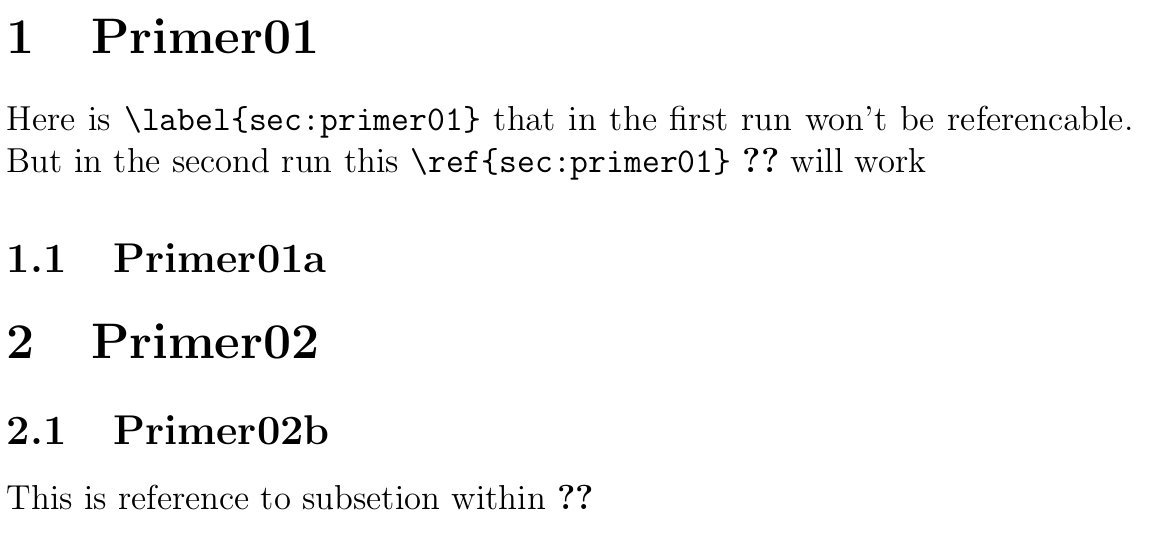
\includegraphics[width=0.5\textwidth]{LabelRef01.png}
    \caption{Label ref first run}
    \label{fig:LabelRef01}
\end{figure}

Later in the second run, this reference will get resolved and the question marks will disappear, but the .aux file will stay the same. You can see this in the figure~\ref{fig:LabelRef02} below.
\begin{figure}[H]
    \centering
    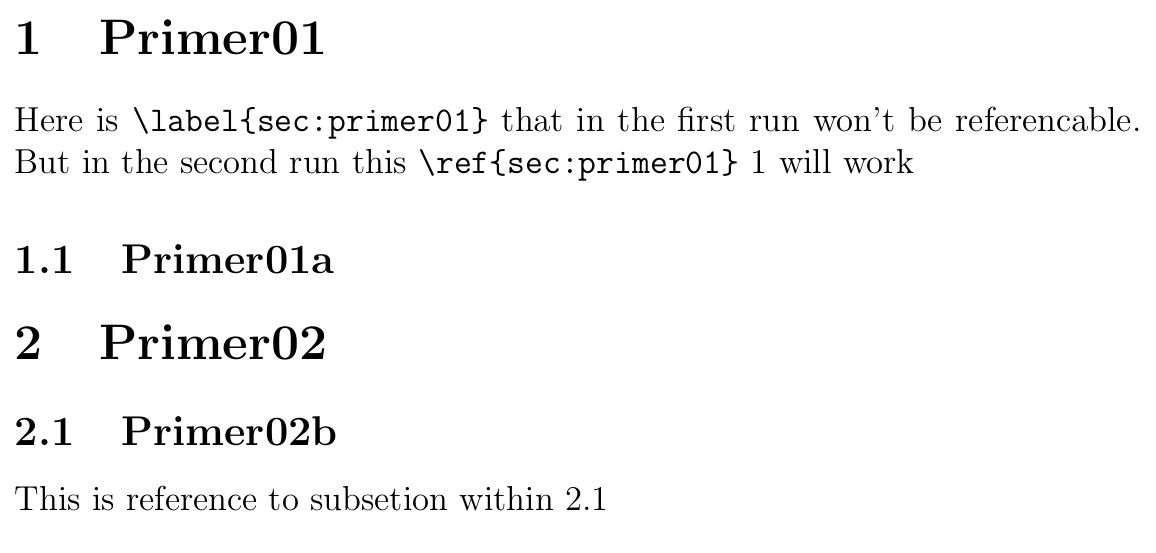
\includegraphics[width=0.5\textwidth]{LabelRef02.png}
    \caption{Label ref second run}
    \label{fig:LabelRef02}
\end{figure}

You can also try out with Primer04. 

\subsection{Include and input files}
First I will explain the motivation behind using \verb|\include{filename}| and \verb|\input{filename}| command. It gives you an opportunity to break large files into a smaller part that you can edit. One huge benefit is that all the settings, formatting and section indexes will be transferred from base file to this included file \cite{Include_input}. This means that you don't need to write twice all the stuff at the top of the file (\verb|\usepackage|, \verb|\graphicspath|, \verb|\newcommand| etc.). This is because when the compiler sees \verb|\include{filename}| or \verb|\input{filename}| command it pauses parsing of the main file and goes to this included file parses it and then continues parsing the main file. \\

The differences between these two commands are that you cannot nest \verb|\include| command in files and that it will force a page break. This makes ideal for book chapters or large seminars. While with \verb|\input| you can nest command in each other files and it will not force a page break. This is ideal for including pictures and making articles. \\

We have also a difference when it comes to .aux files. Let's look at the bottom example. This is Primer05.tex\\

\begin{markdown-block}
    \lstinputlisting{./Primeri/Primer05/Primer05.tex}
\end{markdown-block}

This is Primer05Input.tex\\

\begin{markdown-block}
    \lstinputlisting{./Primeri/Primer05/Primer05Input.tex}
\end{markdown-block}

This is Primer05Include.tex\\
\begin{markdown-block}
    \lstinputlisting{./Primeri/Primer05/Primer05Include.tex}
\end{markdown-block}

Now if we look at Primer05.aux\\
\begin{markdown-block}
    \begin{verbatim}
        \relax 
        \@writefile{toc}{\contentsline {section}{\numberline {1}Input file}{1}}
        \@writefile{lof}{\contentsline {figure}{\numberline {1}{\ignorespaces Input image }}{1}}
        \newlabel{fig:InputImage}{{1}{1}}
        \@input{Primer05Include.aux}
    \end{verbatim}
\end{markdown-block}

we will see that \verb|\include| command makes reference to Primer05Include.aux file. While \verb|\input| command makes direct entry in .aux file. We can see this with at new label.\\
Now let look at Primer05Include.aux file

\begin{markdown-block}
    \begin{verbatim}
        \relax 
        \@writefile{toc}{\contentsline {section}{\numberline {2}Include file}{2}}
        \@writefile{toc}{\contentsline {subsection}{\numberline {2.1}Include subsection}{2}}
        \@writefile{toc}{\contentsline {section}{\numberline {3}Include section 2}{2}}
        \@setckpt{Primer05Include}{
        \setcounter{page}{3}
        \setcounter{equation}{0}
        \setcounter{enumi}{0}
        \setcounter{enumii}{0}
        \setcounter{enumiii}{0}
        \setcounter{enumiv}{0}
        \setcounter{footnote}{0}
        \setcounter{mpfootnote}{0}
        \setcounter{part}{0}
        \setcounter{section}{3}
        \setcounter{subsection}{0}
        \setcounter{subsubsection}{0}
        \setcounter{paragraph}{0}
        \setcounter{subparagraph}{0}
        \setcounter{figure}{1}
        \setcounter{table}{0}
        }
    \end{verbatim}
\end{markdown-block}

We see here that it's the same format as our previous examples. Just that it sets some parameters so that it has right referencing

\section{Infinitely many compiler passes}
When I was researching for this topic I stumbled upon interesting StackExchange question. It was how to write \latex document that would not stabilize (that means it would infinitely many compiles to compile this project). That also means that each compile would give different resoult which is what we don't want.\\
Someone actually answered this question with this document:

\begin{markdown-block}
    \lstinputlisting{./Primeri/Primer06/Primer06.tex}
\end{markdown-block}

The catch here is that when you count pages in Roman numerals, IV take more space than V. This causes to go to a new page. But when on new page it takes less space so it goes back to the old page and this process is cycling forever.\\

If you compile Primer06.tex you will see the result of this. You can also check answer on this \href{https://tex.stackexchange.com/questions/30674/document-requiring-infinitely-many-compiler-passes}{link} \cite{infinitely}

\section{Build Tools}

Now we know how compiling works behind the scenes. Now we can use build tools, editors and online editors that will make our life easier. I will list some of them that are the most popular. And I will only demonstrate only one because in their core each build tool does the same as we would. It executes this chain of commands (pdf)latex -> bibtex/biber -> (pdf)latex -> (pdf)latex -> ... and on each step checks if the document is already stable. This means that it checks if there are some references to resolve and some bibliography to include. 


\textbf{Build tools}\cite{tex_blog}
\begin{itemize}
	\item latexmk - \href{https://mg.readthedocs.io/latexmk.html}{Documentation} home page \cite{latexmk}
	\item Rubber - \href{https://launchpad.net/rubber/}{Home page} \cite{Rubber}
	\item arara - \href{https://github.com/cereda/arara}{Github site} \cite{arara}
\end{itemize}

\textbf{Editors}
*Disclaimer: these editors are specially made for \latex. Almost certainly you could also take your favourite editor and add some plugins and have a functional editor. By favourite editor I have in mind something like (VS Code, Sublime, Eclipse, Emacs, Vim etc.)*
\begin{itemize}
    \item Texmaker - \href{http://www.xm1math.net/texmaker/}{Home page}\cite{texmaker} supported on Linux, Mac and Win
    \item TeXworks - \href{http://www.tug.org/texworks/}{Home page} \cite{texworks} supported on Linux, Mac and Win
    \item TeXShop - \href{https://pages.uoregon.edu/koch/texshop/}{Home page} \cite{texshop} supported on Mac
    \item TeXnicCenter - \href{http://www.texniccenter.org/}{Home page} \cite{texniccenter} supported on Win
\end{itemize}

\textbf{Online Editors}
\begin{itemize}
    \item Overleaf - \href{https://www.overleaf.com/}{Home page} \cite{overleaf}
    \item LaTeX Online Editor (XO) - \href{http://latexonlineeditor.net/}{Home page} \cite{latexonline}
    \item LaTeX Base - \href{https://latexbase.com/}{Home page} \cite{latexbase}
    \item Papeeria - \href{https://papeeria.com/}{Home page} \cite{papeeria}
\end{itemize}

\subsection{Latexmk}
Using Latexmk is as simple as running command:\\

\begin{lstlisting}[language=bash]
    $ latexmk -pdf
\end{lstlisting}

which will run pdflatex on all .tex file in current directory.\\
If you want specific file to be compiled you just add the name like this:\\

\begin{lstlisting}[language=bash]
    $ latexmk myfile.tex -pdf
\end{lstlisting}

and at the end you can clean you directory with this command:\\

\begin{lstlisting}[language=bash]
    $ latexmk -c
\end{lstlisting}

\nocite{*}

\pagebreak

\printbibliography[heading=bibintoc]



\end{document}

% Latex template: Jure Slak, jure.slak@gmail.com
% Dodatki k templatu: Rok Kos, kosrok97@gmail.com